\chapter{Evaluation}
\label{cha:evaluation}

\section{Experimental Setup}
\label{sec:experimental_setup}

The experiments presented in this chapter evaluate the performance of the selected point cloud semantic segmentation architectures on the custom indoor UAV LiDAR dataset introduced in Chapter~\ref{sec:dataset_creation}. The objective is to assess the capability of the different models to distinguish human points from background points and to analyze the trade-off between segmentation performance and computational complexity.

The final dataset consists of 78 valid point clouds acquired in an indoor laboratory environment. Each point cloud contains approximately 50,000 points before sampling and represents a different combination of human pose, subject orientation, occlusion condition, and LiDAR viewpoint. The dataset includes four predefined human poses (standing, sitting, lying down, and T-pose), four subject orientations ($0^\circ$, $90^\circ$, $180^\circ$, and $270^\circ$), and different partial occlusion configurations. The point clouds were manually verified and annotated using the semi-automatic annotation framework described in Section~\ref{subsec:annotation}.

For model training and evaluation, each input sample was represented using only the three-dimensional spatial coordinates (\textit{XYZ}) provided by the LiDAR sensor. A fixed input size of 4096 points per sample was used for all architectures, ensuring a consistent input representation and enabling a fair comparison between models. During training, the sampling strategy combined class-aware sampling and standard random sampling in order to reduce the effect of the strong imbalance between human and background points.

Six point-based semantic segmentation architectures were evaluated: PointNet, PointNet++, DGCNN, PointNeXt-S, PointNeXt-XL, and PointVector. The models cover a range of architectural complexity, from lightweight baseline networks to higher-capacity modern architectures. All models were adapted to the binary segmentation task by replacing the original segmentation head with a two-class output corresponding to \textit{Human} and \textit{Background}.

A transfer learning strategy was employed for all architectures. PointNeXt, DGCNN, and PointVector were initialized using pretrained checkpoints obtained from the OpenPoints framework, while PointNet and PointNet++ were initialized using models pretrained on S3DIS through their corresponding PyTorch implementations. The pretrained networks were subsequently adapted to the three-dimensional input representation and fine-tuned on the custom UAV dataset. All compatible pretrained parameters were allowed to update during the fine-tuning process.

The training procedure used a maximum of 100 epochs with the AdamW optimizer and a batch size of eight. Training was monitored using validation mIoU, with early stopping after 20 consecutive epochs without improvement. A ReduceLROnPlateau learning-rate scheduler was used to reduce the learning rate when validation performance stagnated. The model corresponding to the highest validation mIoU was retained for subsequent evaluation. Data augmentation included random rotations around the vertical axis, scaling, translation, coordinate jittering, and random point dropout.

All experiments were conducted using an NVIDIA GeForce RTX 4050 GPU. PointNeXt, DGCNN, and PointVector were implemented using the OpenPoints framework, while PointNet and PointNet++ were evaluated using their official PyTorch implementations. The complete training configuration is described in Section~\ref{subsec:training_configuration}.

The quantitative evaluation focuses primarily on semantic segmentation performance, while computational performance is analyzed separately in Section~\ref{sec:computational_performance}. This separation allows the segmentation accuracy of the different architectures to be assessed independently before considering their computational requirements and suitability for the intended UAV perception system.

\section{Quantitative Evaluation of the Segmentation Models}
\label{subsec:quantitative_results}
The quantitative evaluation was performed using both the validation and held-out test splits of the custom UAV LiDAR dataset. The validation set was used during training to monitor model performance and select the best checkpoint for each architecture, whereas the held-out test set provides the primary basis for the final comparison, as it evaluates the models on previously unseen scenes.

Since the task is formulated as binary semantic segmentation between \textit{background} and \textit{person}, overall accuracy and mean Intersection over Union (mIoU) were considered together with class-specific IoU, precision, recall, and F1-score. Particular emphasis was placed on the \textit{person} class, since the predominance of background points can make overall accuracy insufficient to characterize the quality of human segmentation.

\subsection{Validation Results}

Table~\ref{tab1} summarizes the performance obtained on the validation set. PointVector achieves the highest validation performance, with an mIoU of 0.9426, a person IoU of 0.8969, and a person F1-score of 0.9457. PointNeXt-XL follows with an mIoU of 0.9322 and a person IoU of 0.8780, while the remaining architectures obtain lower values.

\begin{table}[H]
\centering
\caption{Quantitative validation results obtained by the evaluated segmentation models.}
\label{tab1}
\resizebox{\textwidth}{!}{
\begin{tabular}{|l|c|c|c|c|c|c|}
\hline
\textbf{Model} &
\textbf{Accuracy} &
\textbf{mIoU} &
\textbf{Person IoU} &
\textbf{Person Precision} &
\textbf{Person Recall} &
\textbf{Person F1} \\
\hline
PointNet & 0.9823 & 0.9016 & 0.8224 & 0.8565 & 0.9539 & 0.9026 \\
\hline
PointNet++ & 0.9800 & 0.9015 & 0.8251 & 0.8548 & 0.9595 & 0.9041 \\
\hline
DGCNN & 0.9844 & 0.9126 & 0.8422 & 0.8782 & 0.9536 & 0.9144 \\
\hline
PointNeXt-S & 0.9843 & 0.9129 & 0.8431 & 0.8827 & 0.9494 & 0.9148 \\
\hline
PointNeXt-XL & 0.9876 & 0.9322 & 0.8780 & 0.8997 & 0.9733 & 0.9351 \\
\hline
\textbf{PointVector} & \textbf{0.9894} & \textbf{0.9426} & \textbf{0.8969} & \textbf{0.9068} & \textbf{0.9880} & \textbf{0.9457} \\
\hline
\end{tabular}
}
\end{table}

The validation results indicate a progressive improvement from the PointNet-based baselines towards the more recent architectures. In particular, PointNeXt-XL substantially improves over PointNeXt-S, while PointVector obtains the best validation scores across the reported metrics. However, these results are used primarily to characterize model performance during development. The final assessment is based on the independent test set.

The class-specific validation results in Table~\ref{tab2} show that the \textit{person} class is consistently more challenging than the background. All models achieve background IoU values above 0.97, whereas person IoU ranges from 0.8224 to 0.8969. This difference is expected due to the smaller proportion of human points and the geometric complexity and partial occlusions associated with the human class.

\begin{table}[H]
\centering
\caption{Class-specific validation performance for the evaluated models.}
\label{tab2}
\resizebox{\textwidth}{!}{
\begin{tabular}{|l|c|c|c|c|c|c|c|c|}
\hline
\textbf{Model} &
\multicolumn{4}{c|}{\textbf{Background}} &
\multicolumn{4}{c|}{\textbf{Person}} \\
\cline{2-9}
&
\textbf{IoU} & \textbf{Prec.} & \textbf{Recall} & \textbf{F1} &
\textbf{IoU} & \textbf{Prec.} & \textbf{Recall} & \textbf{F1} \\
\hline
PointNet
& 0.9807 & 0.9956 & 0.9850 & 0.9903
& 0.8224 & 0.8565 & 0.9539 & 0.9026 \\
\hline
PointNet++
& 0.9780 & 0.9955 & 0.9823 & 0.9889
& 0.8251 & 0.8548 & 0.9595 & 0.9041 \\
\hline
DGCNN
& 0.9829 & 0.9955 & 0.9873 & 0.9914
& 0.8422 & 0.8782 & 0.9536 & 0.9144 \\
\hline
PointNeXt-S
& 0.9828 & 0.9950 & 0.9877 & 0.9913
& 0.8431 & 0.8827 & 0.9494 & 0.9148 \\
\hline
PointNeXt-XL
& 0.9864 & 0.9973 & 0.9890 & 0.9931
& 0.8780 & 0.8997 & 0.9733 & 0.9351 \\
\hline
\textbf{PointVector}
& \textbf{0.9883} & \textbf{0.9988} & \textbf{0.9895} & \textbf{0.9941}
& \textbf{0.8969} & \textbf{0.9068} & \textbf{0.9880} & \textbf{0.9457} \\
\hline
\end{tabular}
}
\end{table}

\subsection{Held-Out Test Results}

The final evaluation was performed on a held-out test split consisting of eight previously unseen scenes, corresponding to 160 samples and 655,360 evaluated points. 4096 points per sample, and no data augmentation were used during testing.

The test results are presented in Table~\ref{tab3}. Unlike the validation results, where PointVector achieved the highest scores, the held-out test set identifies PointNeXt-XL as the best-performing architecture. This result is particularly important because the test set provides the most direct assessment of the models' ability to generalize to unseen UAV LiDAR scenes.

\begin{table}[ht]
\centering
\caption{Quantitative test-set performance of the evaluated semantic segmentation models.}
\label{tab3}
\begin{tabular}{lcccccc}
\hline
Model & Accuracy & mIoU & Person IoU & Person P. & Person R. & Person F1 \\
\hline
\textbf{PointNeXt-XL} & \textbf{0.9896} & \textbf{0.9377} & \textbf{0.8866} & \textbf{0.8906} & \textbf{0.9949} & \textbf{0.9399} \\
PointVector & 0.9879 & 0.9282 & 0.8697 & 0.8730 & 0.9957 & 0.9303 \\
PointNeXt-S & 0.9824 & 0.8992 & 0.8174 & 0.8397 & 0.9686 & 0.8996 \\
DGCNN & 0.9769 & 0.8745 & 0.7740 & 0.7928 & 0.9703 & 0.8726 \\
PointNet & 0.9751 & 0.8673 & 0.7616 & 0.7760 & 0.9763 & 0.8647 \\
PointNet++ & 0.9725 & 0.8554 & 0.7407 & 0.7606 & 0.9659 & 0.8510 \\
\hline
\end{tabular}
\end{table}

PointNeXt-XL achieves the highest test performance across the main evaluation metrics, obtaining an accuracy of 0.9896, an mIoU of 0.9377, a person IoU of 0.8866, and a person F1-score of 0.9399. Its person recall reaches 0.9949, indicating that the model successfully identifies almost all human points in the unseen test scenes. PointVector obtains the second-best overall results, with an mIoU of 0.9282, a person IoU of 0.8697, and a person F1-score of 0.9303. Although PointVector achieves a marginally higher person recall (0.9957), PointNeXt-XL outperforms it in accuracy, mIoU, person IoU, precision, and F1-score.

The test results also reveal an important difference between validation performance and generalization. PointVector achieves the highest validation mIoU (0.9426), but its performance decreases to 0.9282 on the test set. Its person IoU similarly decreases from 0.8969 to 0.8697. In contrast, PointNeXt-XL maintains highly consistent performance, with its mIoU changing from 0.9322 on validation to 0.9377 on test, while its person IoU increases from 0.8780 to 0.8866. Its F1-score also remains stable, changing from 0.9351 to 0.9399.

The remaining models show a clearer performance degradation on unseen scenes. PointNet and PointNet++ obtain test person IoU values of 0.7616 and 0.7407, respectively, while DGCNN reaches 0.7740. PointNeXt-S performs better, with a person IoU of 0.8174, but remains below PointNeXt-XL. These results suggest that the increased representational capacity of PointNeXt-XL provides a more robust representation of the geometric characteristics required for human segmentation in unseen scenes.

Overall, the held-out test evaluation provides the main evidence for the final model comparison. Although PointVector achieves the best validation performance, PointNeXt-XL achieves the best results on the independent test set and exhibits the most consistent performance between validation and unseen data. Therefore, PointNeXt-XL is selected as the best-performing architecture in terms of segmentation quality and generalization.

This test-based selection is particularly relevant for the intended UAV application, where performance on previously unseen scenes is more representative of real deployment conditions than performance on the validation set. The final model selection will therefore consider PointNeXt-XL as the reference architecture, with computational requirements and inference performance analyzed subsequently to determine its suitability for deployment on the aerial platform.

\section{Qualitative Results}
\label{sec:qualitative_results}

In addition to the quantitative evaluation, a qualitative analysis was performed to visually examine the behavior of the trained segmentation models on representative indoor LiDAR scenes. The analysis focuses not only on the ability of the models to identify the human subject, but also on their failure modes, particularly false positive predictions in regions where no human is present.

Figure~\ref{fig:qualitative_normal} presents a representative acquisition in which the human subject is clearly visible. Most architectures are able to recover the main structure of the person, although noticeable differences can be observed in the amount of background incorrectly classified as human. In particular, PointNet produces a comparatively large number of false positive predictions around the scene. This behavior was also observed repeatedly during the qualitative inspection, indicating a tendency of this architecture to classify geometrically similar background points as part of the human class.

\begin{figure}[H]
\centering
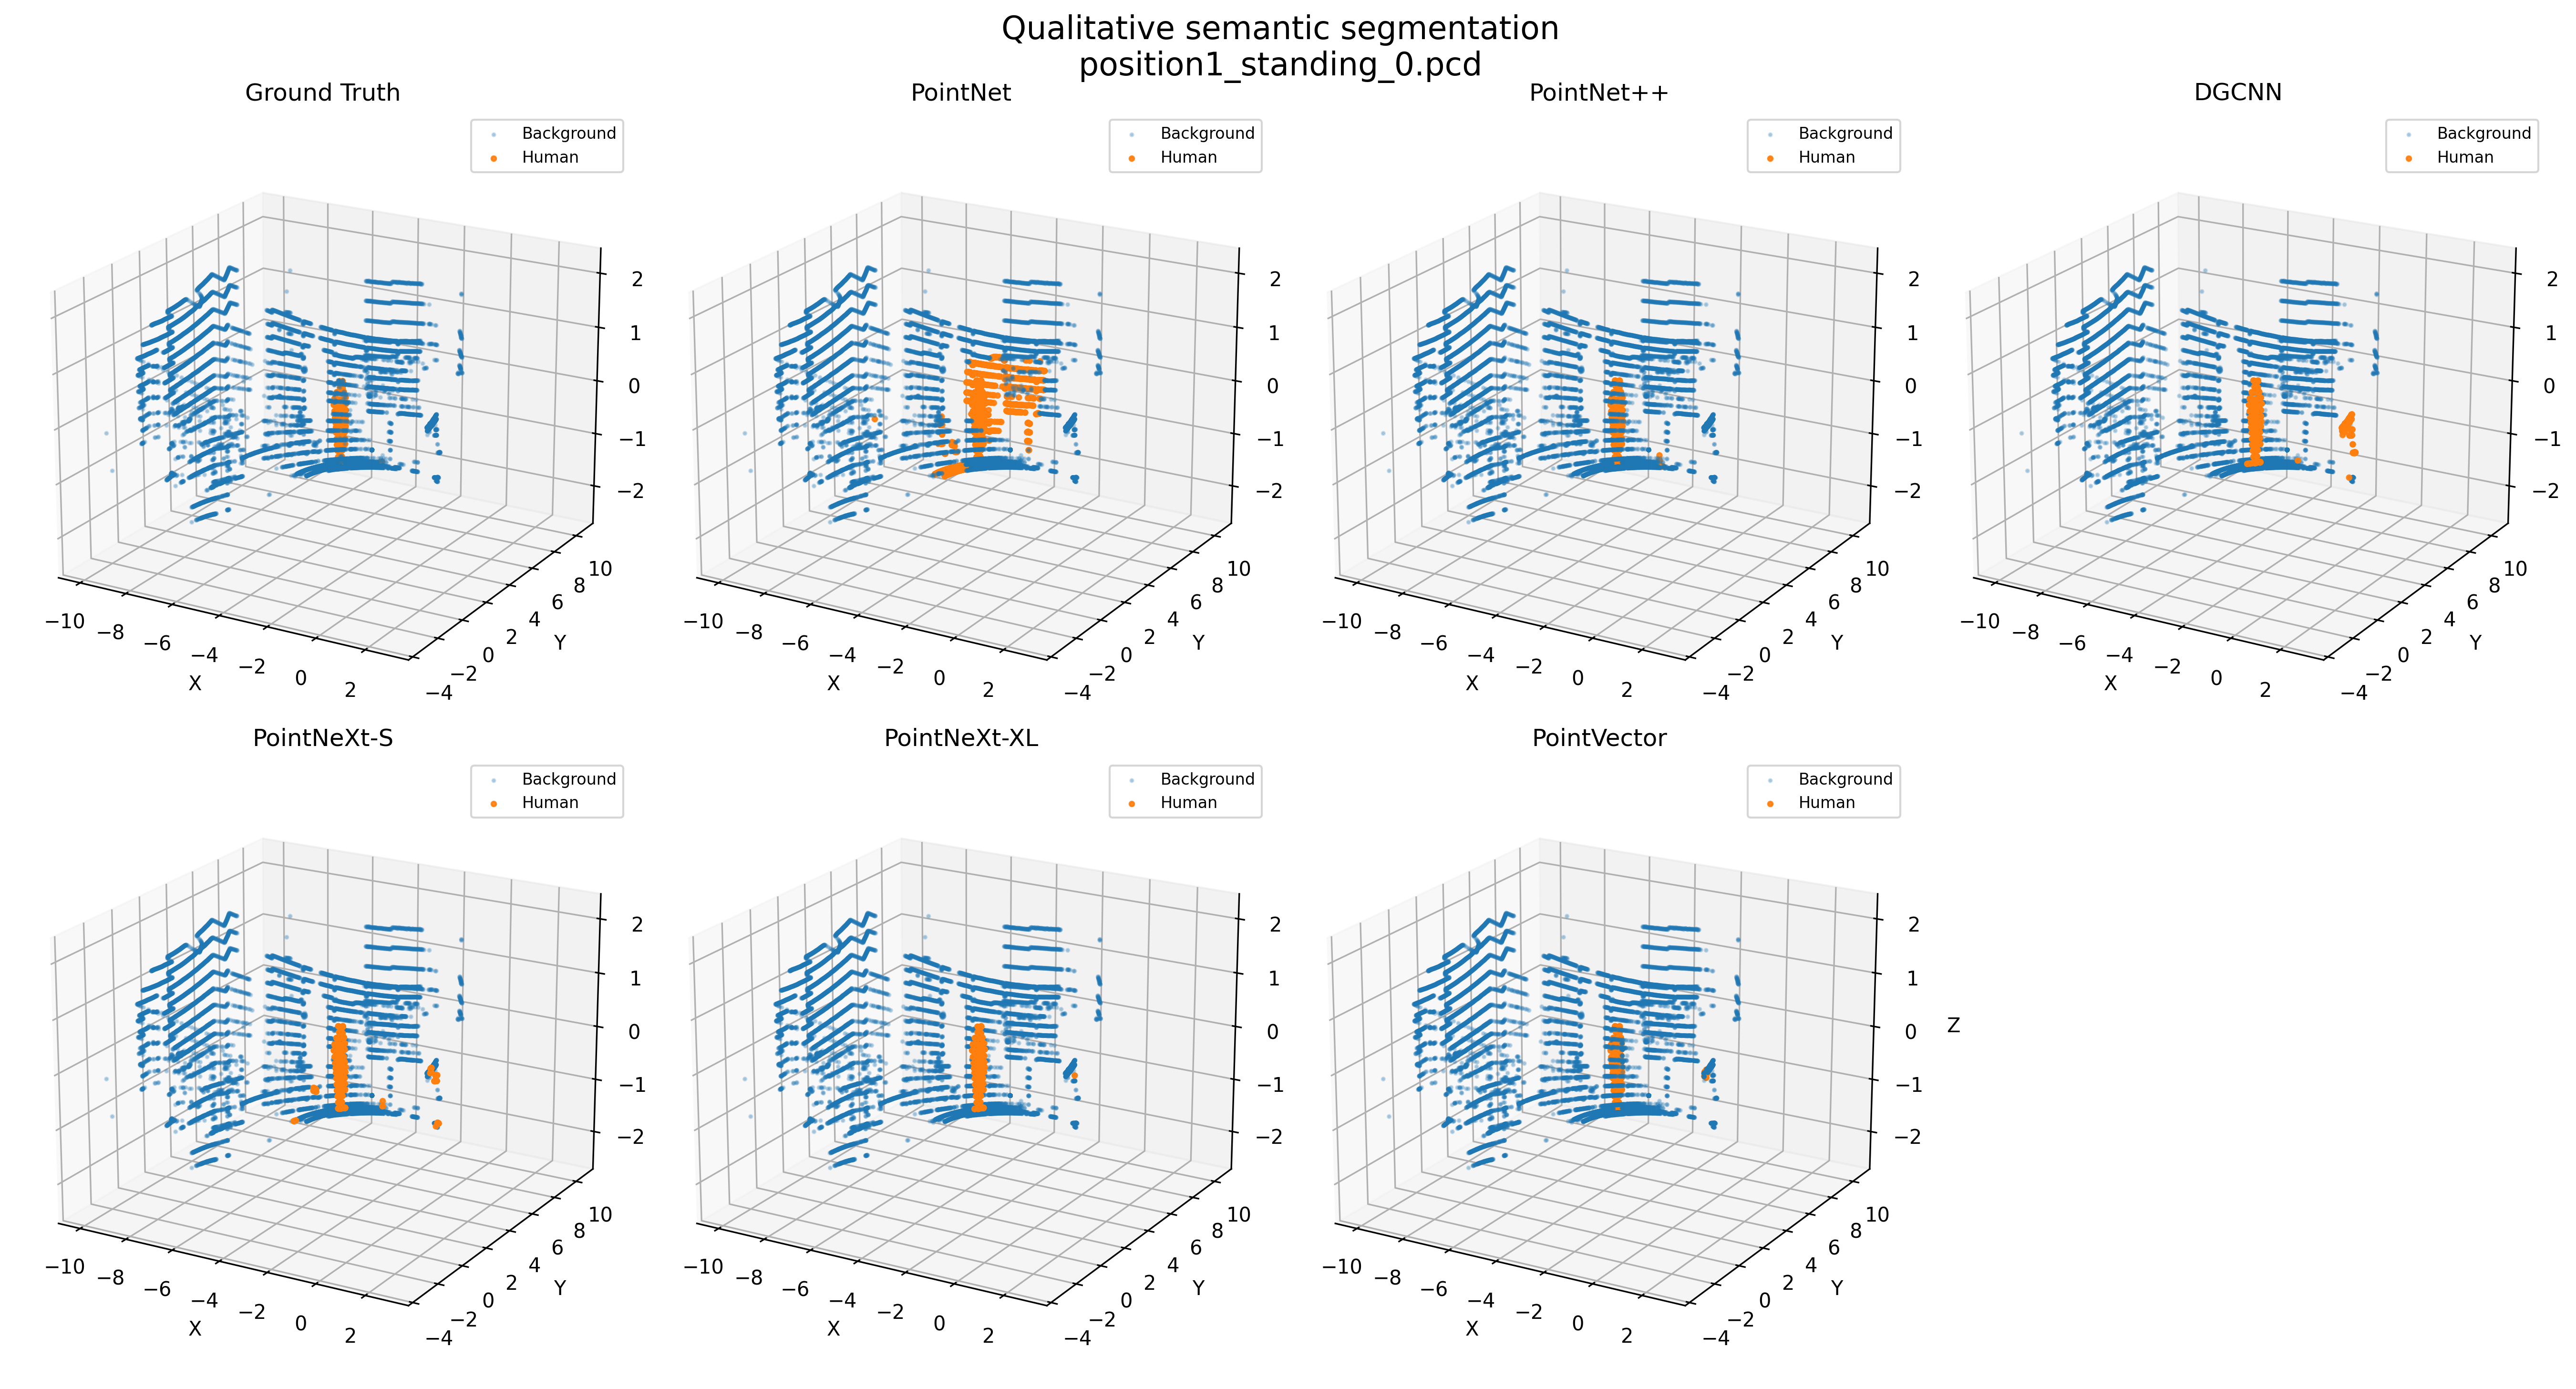
\includegraphics[width=\textwidth]{qualitative_results.png}
\caption{Qualitative segmentation results for a representative indoor scene with a clearly visible human subject. The ground-truth annotation is compared with the predictions produced by the evaluated architectures. PointNet exhibits a comparatively large number of false positive human predictions.}
\label{fig:qualitative_normal}
\end{figure}

A more challenging configuration is presented in Figure~\ref{fig:qualitative_occlusion}, where the human subject is substantially occluded by the experimental barriers. Only a limited portion of the body is visible to the LiDAR sensor, making the distinction between human and background considerably more ambiguous. In this situation, the evaluated models tend to produce additional human predictions in regions where no corresponding ground-truth points are present. This effect is particularly pronounced for the architectures with poorer quantitative performance, which generate larger and more spatially dispersed false positive regions.

\begin{figure}[H]
\centering
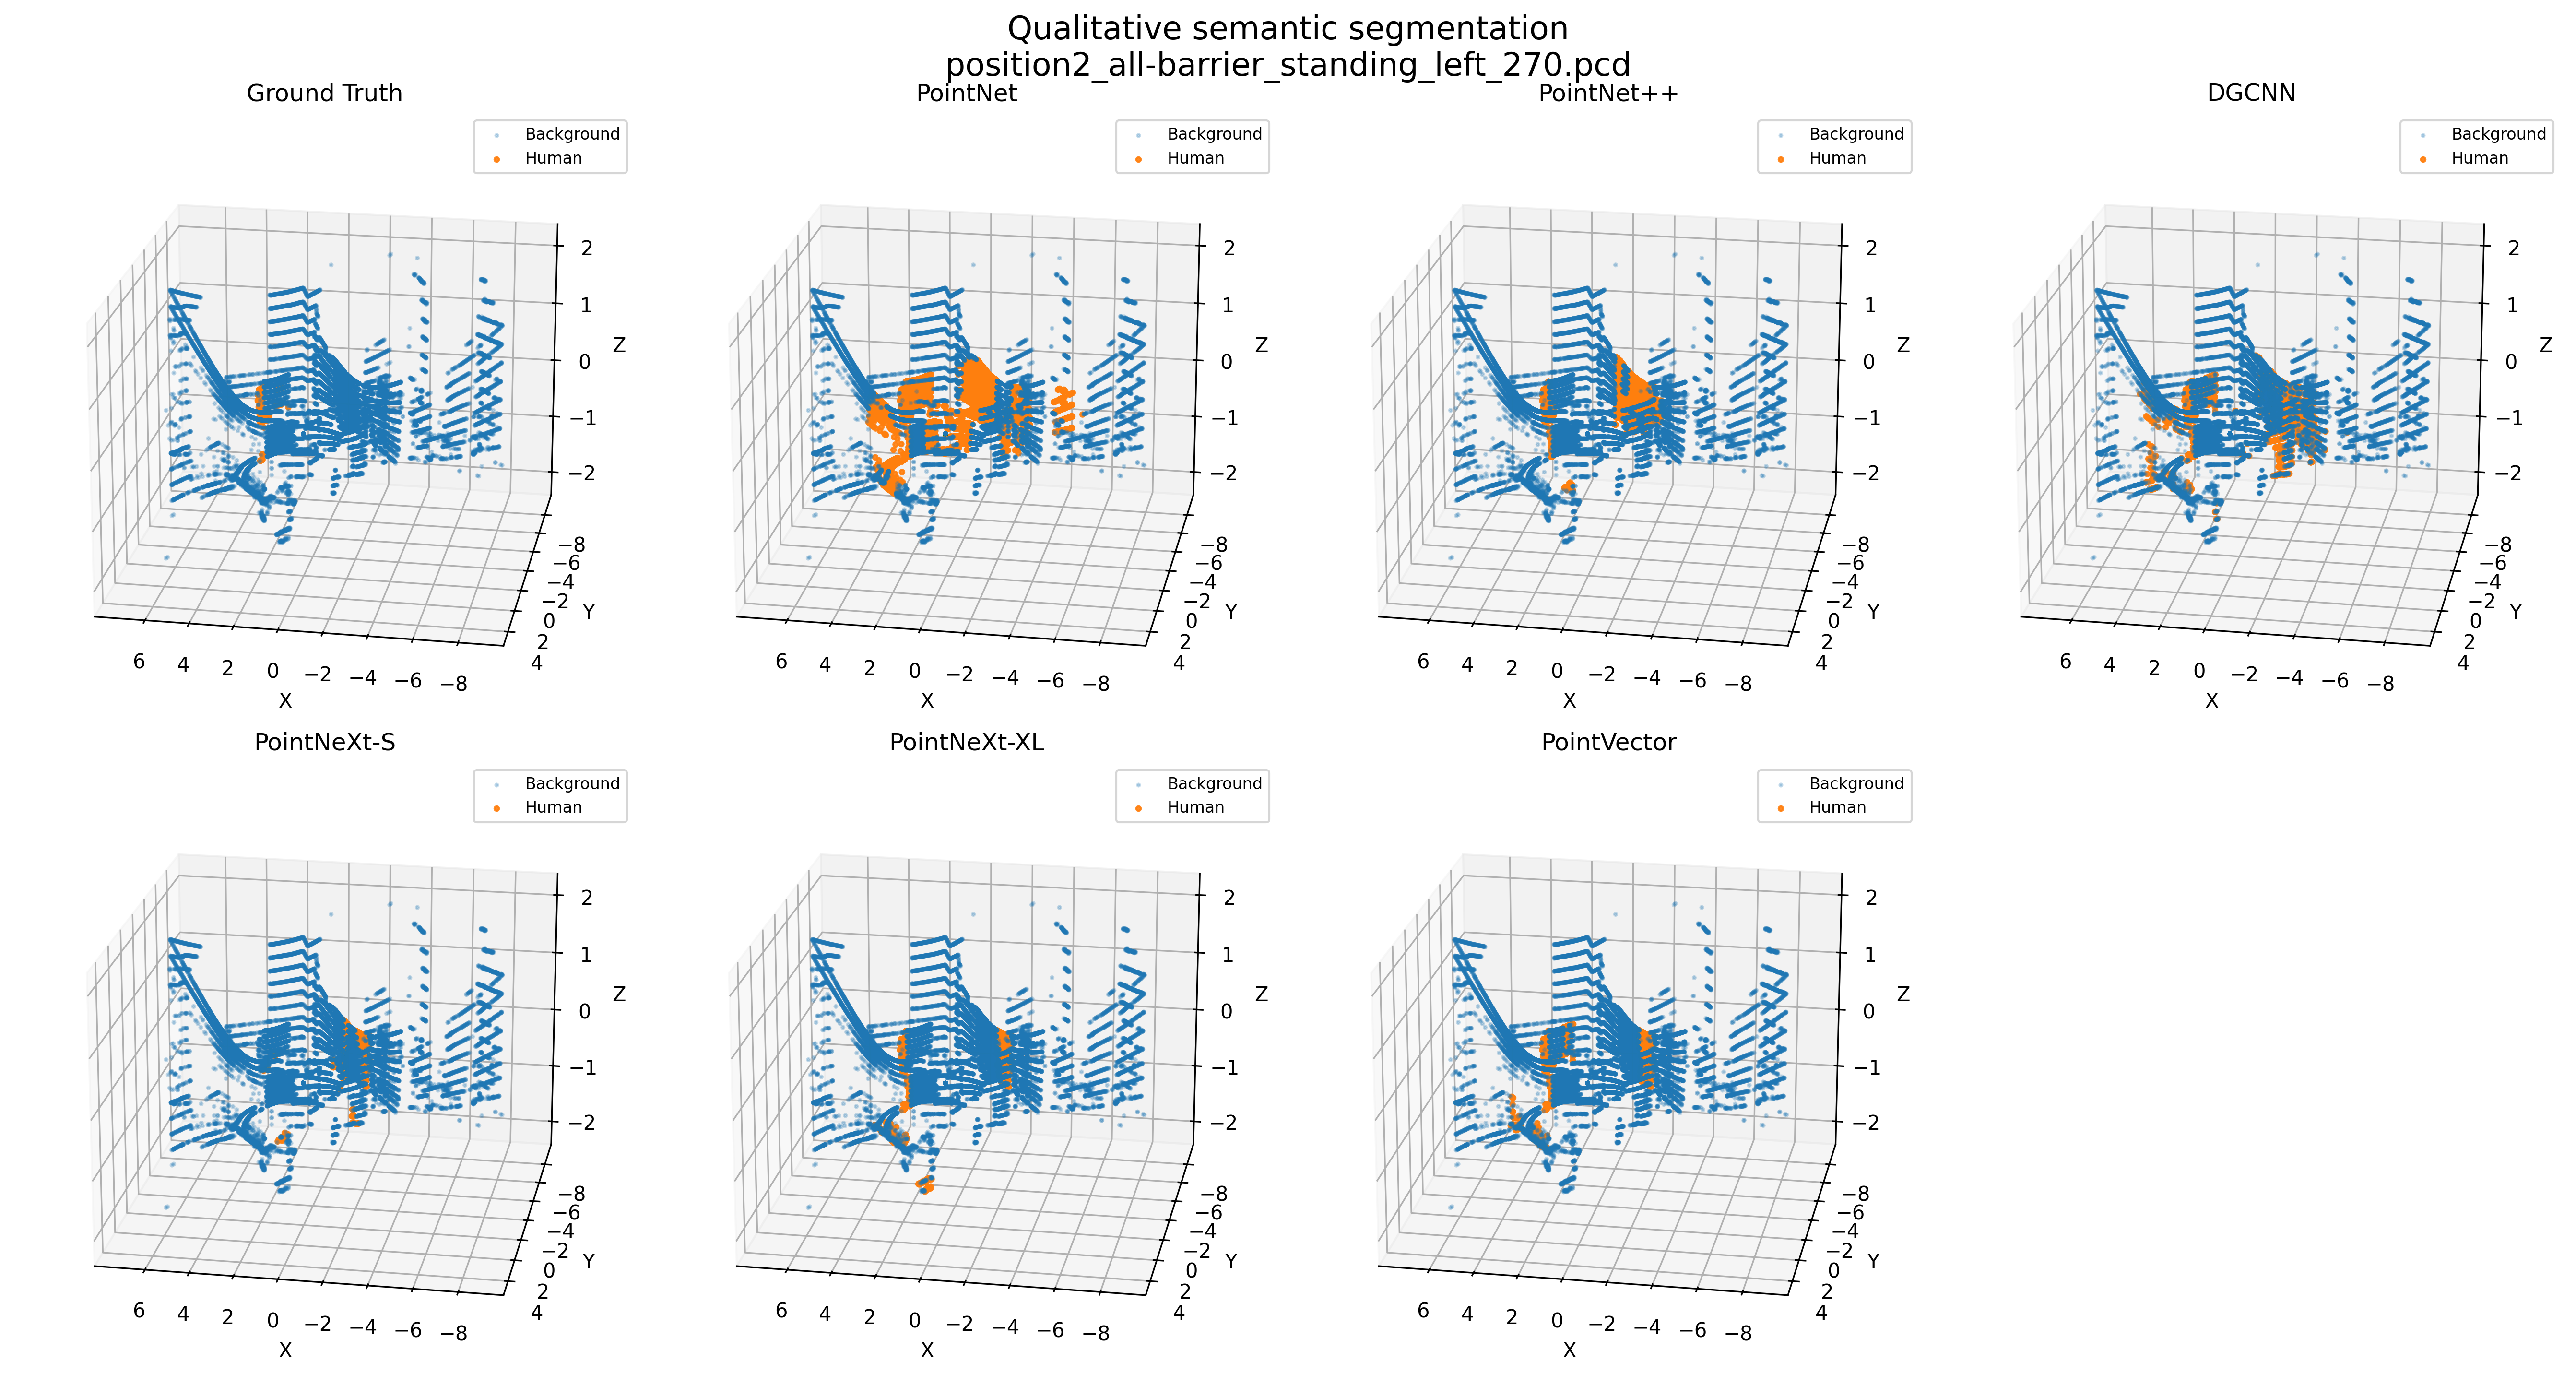
\includegraphics[width=\textwidth]{qualitative_results2.png}
\caption{Qualitative segmentation results for a heavily occluded human subject. The reduced amount of visible human geometry increases the number of false positive predictions, particularly for the less accurate models.}
\label{fig:qualitative_occlusion}
\end{figure}

To further investigate this behavior, a third example is presented in Figure~\ref{fig:qualitative_empty}, corresponding to a scene containing no human subject. In this case, the ground truth contains no human points; nevertheless, all evaluated architectures produce some predictions belonging to the \textit{Human} class. This provides a clear illustration of the false positive behavior observed during the experiments. Background structures or isolated geometric patterns can therefore be incorrectly interpreted as parts of a human body, even when no human is present in the scene.

\begin{figure}[H]
\centering
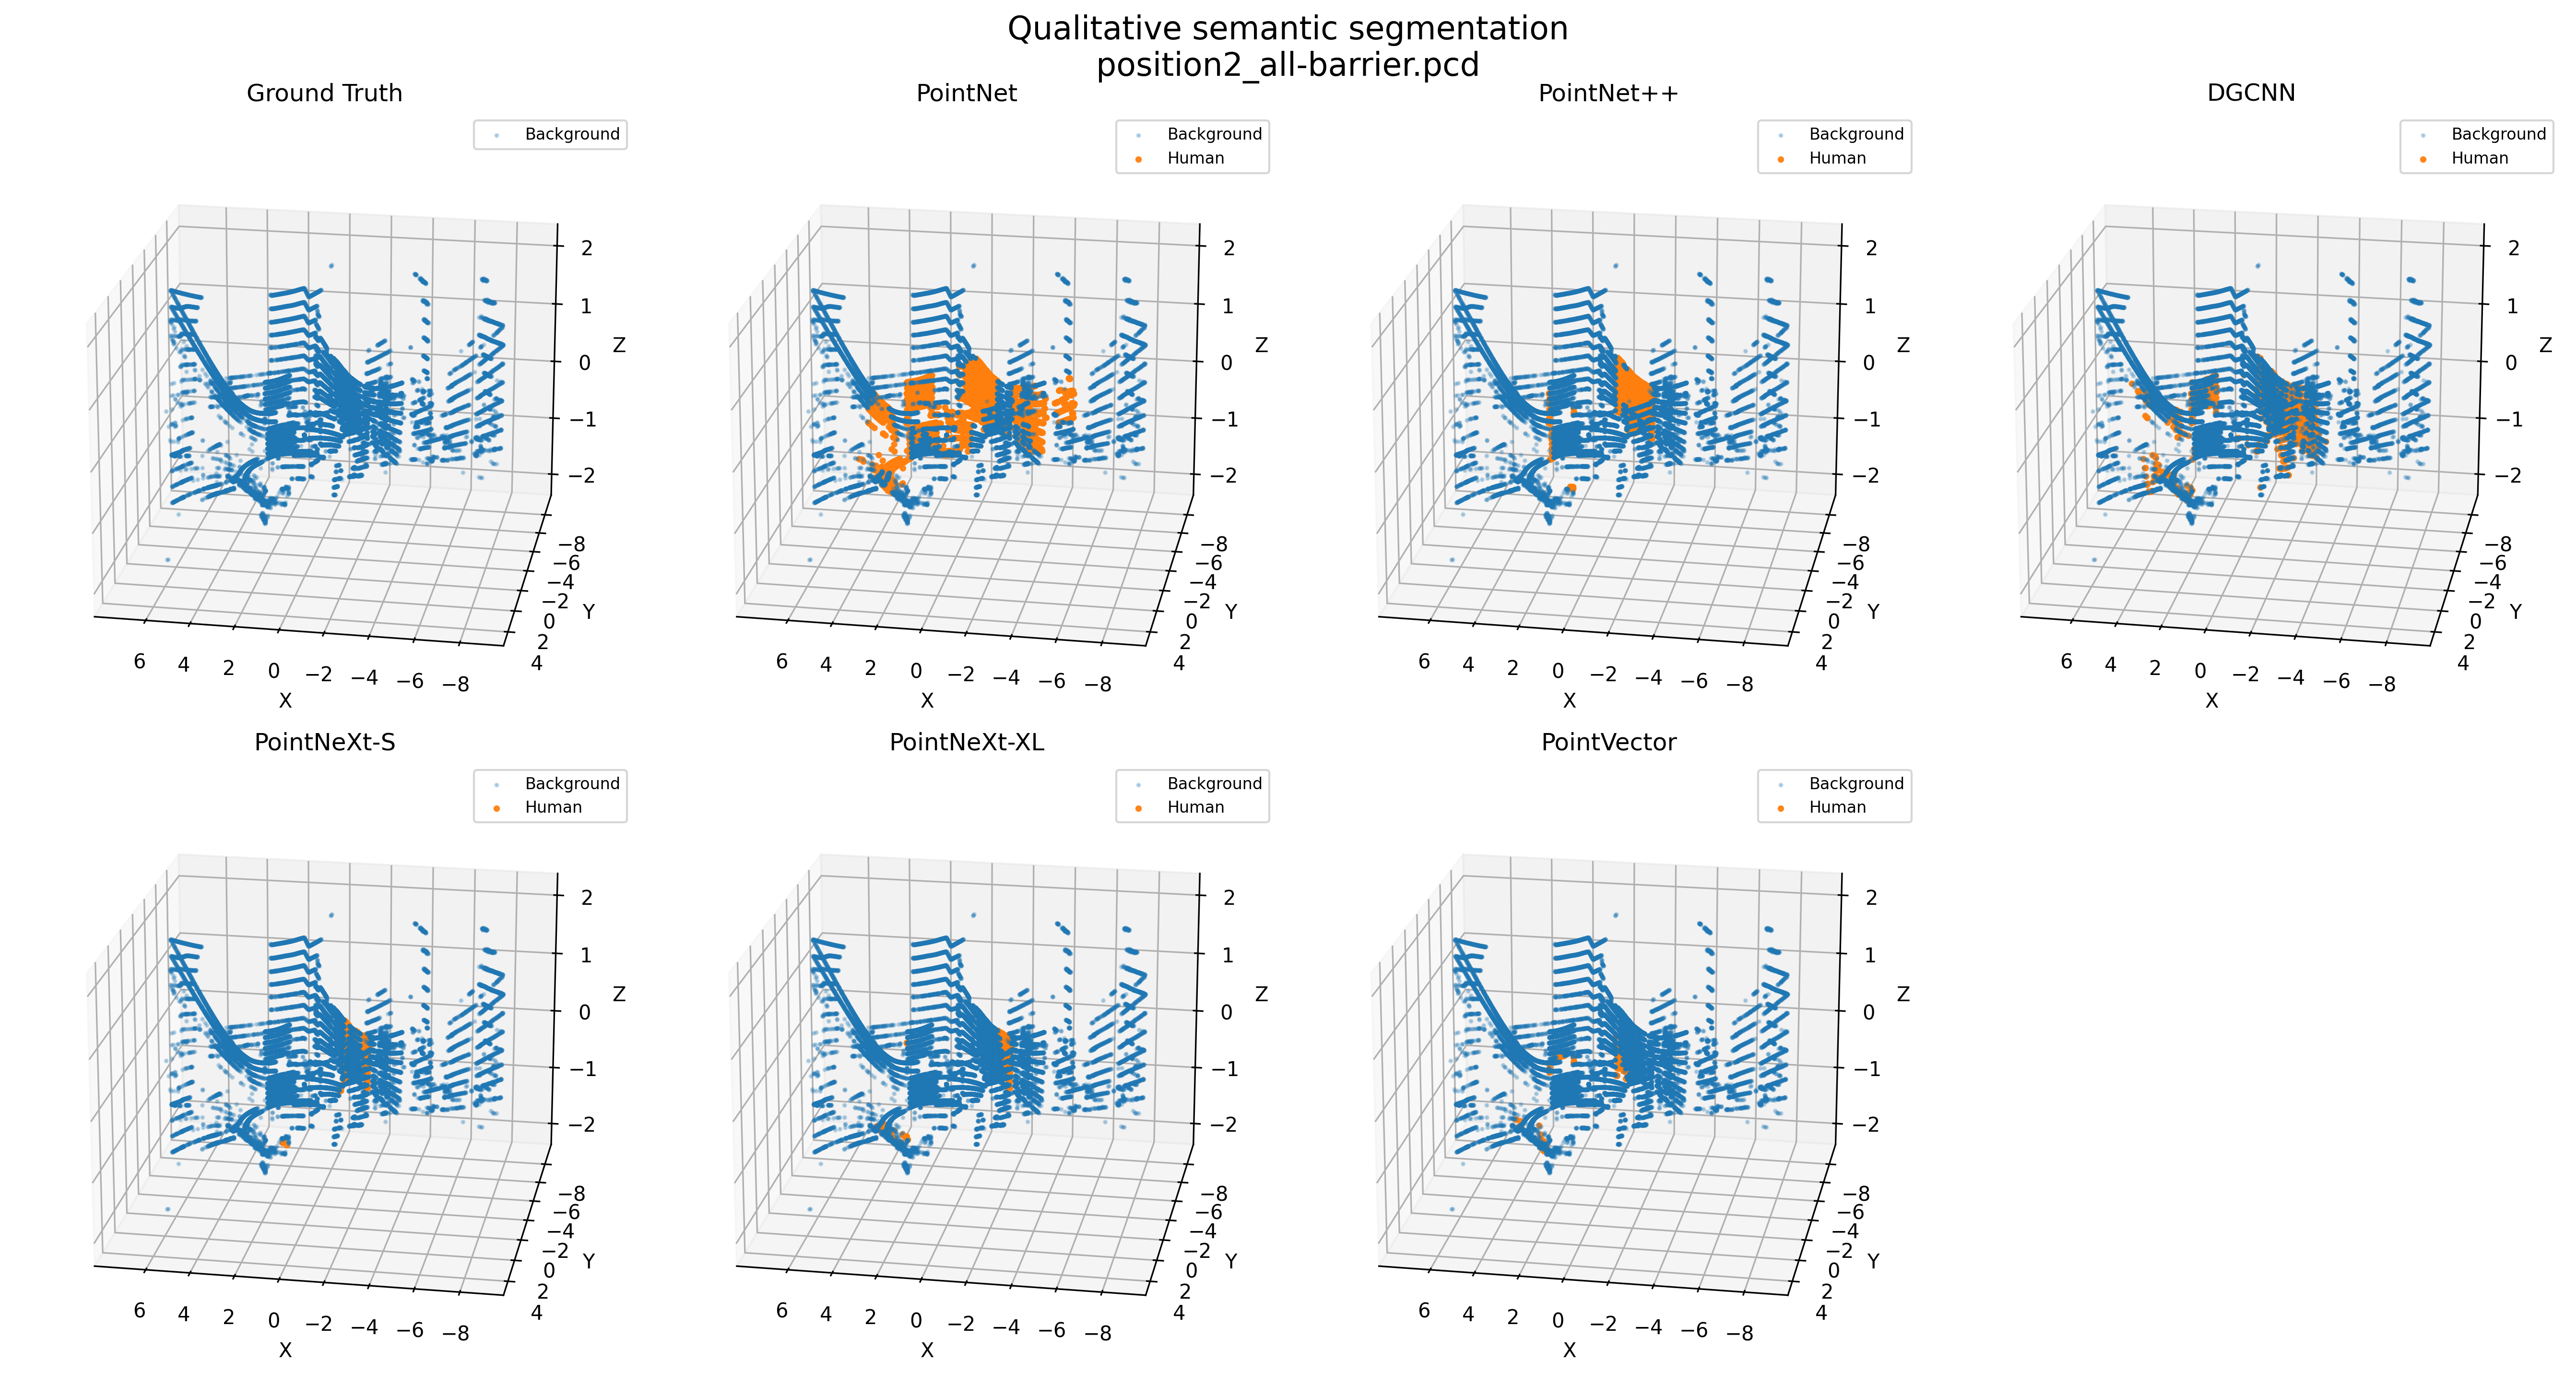
\includegraphics[width=\textwidth]{qualitative_results3.png}
\caption{Qualitative segmentation results for an indoor scene without a human subject. Although the ground truth contains no human points, all evaluated models produce false positive human predictions.}
\label{fig:qualitative_empty}
\end{figure}

These examples highlight an important limitation of the evaluated models. Although the networks are capable of identifying human structures in favorable conditions, their predictions become less reliable when the available geometric evidence is incomplete or when background structures exhibit shapes that are compatible with human geometry. This limitation is particularly relevant for UAV-based perception, where changes in viewpoint and partial occlusion can result in incomplete observations of the target.

Overall, the qualitative analysis complements the quantitative results presented in Section~\ref{subsec:quantitative_results}. Rather than demonstrating only successful detections, the selected examples illustrate the main error patterns identified during evaluation, with false positive predictions representing a relevant source of error across the evaluated architectures. The qualitative results therefore reinforce the importance of considering both segmentation accuracy and robustness to background geometry and partial observations when assessing the suitability of the models for indoor UAV perception.

\section{Computational Performance}
\label{sec:computational_performance}

In addition to the segmentation accuracy, the computational cost of the evaluated architectures was assessed by performing a standalone-style inference experiment over the complete custom dataset. The objective of this experiment was to characterize the practical inference performance of each model under the same hardware and software conditions and to evaluate its suitability for the intended UAV perception pipeline.

The benchmark was performed on the complete set of 78 point clouds contained in the cleaned dataset. Since the point clouds contain a substantially larger number of points than the fixed input size used by the networks, each cloud was divided into 4096-point patches. The predictions obtained for the individual patches were processed sequentially to cover the complete point cloud. In total, the 78 acquisitions contained 3,631,106 points and resulted in 931 patches across the complete dataset. The same inference procedure was applied to all six evaluated architectures.

The benchmark was executed using the NVIDIA GeForce RTX 4050 GPU employed throughout the training and evaluation process. The models were loaded from their final \texttt{best\_model} checkpoints and inference was performed using the same implementations employed during model development. A warm-up stage was performed before processing the dataset in order to reduce the influence of the initial CUDA execution overhead. The reported inference time therefore corresponds to the processing of the dataset after model initialization and warm-up.

Table~\ref{tab:inference_performance} summarizes the resulting computational performance.

\begin{table}[H]
\centering
\caption{Inference performance over the complete custom LiDAR dataset.}
\label{tab:inference_performance}
\begin{tabular}{|l|r|r|r|r|}
\hline
\textbf{Model} &
\textbf{Total Inference (s)} &
\textbf{Mean Cloud (s)} &
\textbf{Points/s} &
\textbf{Patches/s} \\
\hline
PointNet & 3.0191 & 0.0387 & 1,202,730.57 & 308.37 \\
\hline
PointNet++ & 112.4955 & 1.4422 & 32,277.80 & 8.28 \\
\hline
DGCNN & 37.9691 & 0.4868 & 95,633.24 & 24.52 \\
\hline
PointNeXt-S & 3.7066 & 0.0475 & 979,620.09 & 251.17 \\
\hline
PointNeXt-XL & 14.5317 & 0.1863 & 249,875.66 & 64.07 \\
\hline
PointVector & 11.3189 & 0.1451 & 320,800.15 & 82.25 \\
\hline
\end{tabular}
\end{table}

The results show substantial differences in computational requirements between the evaluated architectures. PointNet achieved the lowest total inference time, requiring only 3.02~s to process the complete dataset, with an average processing time of 38.7~ms per point cloud. Its throughput reached approximately 1.20 million points per second. PointNeXt-S exhibited very similar behavior, requiring 3.71~s for the complete dataset and processing approximately 980,000 points per second. These results confirm the computational advantage of lightweight point-based architectures.

DGCNN required 37.97~s to process the complete dataset, corresponding to an average of 486.8~ms per point cloud. Its throughput was approximately 95,633 points per second, substantially lower than that of PointNet and PointNeXt-S. This difference is consistent with the additional computational cost associated with dynamically constructing and processing local feature relationships.

The larger PointNeXt-XL model required 14.53~s for the complete dataset, while PointVector required 11.32~s. Their average processing times were 186.3~ms and 145.1~ms per point cloud, respectively. Although both architectures are considerably more computationally demanding than PointNet and PointNeXt-S, their inference requirements remain substantially lower than those observed for PointNet++ in the evaluated configuration.

PointNet++ exhibited the highest computational cost among the evaluated models by a significant margin. Processing the complete dataset required 112.50~s, corresponding to an average of 1.44~s per point cloud and a throughput of approximately 32,278 points per second. However, this result must be interpreted in the context of the specific implementation used in this work. PointNet++ was evaluated using the PyTorch-based implementation employed during development, which does not make use of the same CUDA-optimized operations available in the OpenPoints-based implementations used for the other evaluated architectures. Consequently, the measured latency includes additional computational overhead associated with the underlying implementation and should not be interpreted as a direct measure of the intrinsic computational complexity of the PointNet++ architecture alone.

In contrast, DGCNN, PointNeXt-S, PointNeXt-XL, and PointVector were evaluated using their OpenPoints implementations with CUDA acceleration. Therefore, the comparison between these models provides a more direct indication of their relative computational requirements under GPU-accelerated execution. PointNet was also evaluated using its dedicated PyTorch implementation, as described in Section~\ref{subsec:training_environment}.

It is important to note that these measurements represent model inference over already reconstructed point clouds. The reported latency therefore does not include LiDAR acquisition, packet decoding, point cloud generation, preprocessing, Wi-Fi transmission, or other system-level processing stages. These operations have not been included in the model-specific latency comparison because they are common to the perception pipeline and do not depend on the neural network architecture being evaluated. Including them would therefore obscure the differences in computational cost attributable specifically to the segmentation models.

Consequently, the reported values should be interpreted as the computational component of the semantic segmentation stage rather than as an end-to-end UAV perception latency. The benchmark nevertheless provides a useful comparison of the computational requirements of the evaluated architectures under the intended external GPU-based inference configuration.

Overall, PointNet and PointNeXt-S provide the most favorable inference performance, requiring approximately 3~s to process the complete dataset. PointVector and PointNeXt-XL provide intermediate computational requirements, while DGCNN presents a substantially higher inference cost. PointNet++ exhibits the highest measured latency in the evaluated configuration, although its result is strongly influenced by the non-CUDA-optimized PyTorch implementation used for inference. These results are particularly relevant to the deployment strategy adopted in this work, where deep learning inference is performed on an external GPU-equipped workstation rather than directly on the Raspberry Pi. The benchmark therefore characterizes the model-dependent computational cost of the proposed segmentation stage while providing a reference for future optimization and edge deployment studies.


\section{Discussion}
\label{sec:discussion}

The results obtained throughout the experimental evaluation provide a clear indication of the relative suitability of the evaluated architectures for the proposed aerial LiDAR segmentation system. Although the models exhibit different strengths depending on the evaluation criterion, the combined analysis of segmentation quality, qualitative behavior, and computational cost identifies PointNeXt-S as the most favorable overall configuration for the intended application.

From a computational perspective, PointNeXt-S provides the best balance among the evaluated architectures. It processed the complete dataset in 3.71~s, corresponding to an average of 47.5~ms per point cloud and a throughput of approximately 980,000 points per second. These values are very close to those obtained by PointNet, which achieved the lowest absolute inference time, while PointNeXt-S provides a more modern feature extraction architecture and achieves competitive segmentation performance. The relatively small difference in inference time between both models is particularly relevant for the intended application, since it indicates that the additional representational capacity of PointNeXt-S does not introduce a significant computational penalty in the evaluated configuration.

The remaining architectures present substantially higher computational requirements. DGCNN requires 37.97~s to process the complete dataset, while PointNeXt-XL and PointVector require 14.53~s and 11.32~s, respectively. PointNet++ represents the most computationally demanding configuration, requiring 112.50~s for the same experiment. In the present implementation, PointNet++ does not take advantage of the same CUDA-optimized execution path as the other architectures and relies more heavily on standard PyTorch operations. Consequently, its measured latency should not be interpreted exclusively as an intrinsic limitation of the PointNet++ architecture, but rather as the computational cost of the specific implementation evaluated in this work. Nevertheless, the measurement remains relevant because it represents the actual configuration used in the experimental system and because it will never be faster than PointNet because it is an iteration of the latter.

The qualitative evaluation provides an additional perspective on the differences between architectures. In relatively straightforward scenes, the evaluated models are generally capable of recovering the main structure of the human subject. However, false positive predictions are visible in some configurations, particularly for PointNet. This behavior becomes more evident in scenes where the background contains geometric structures that can be confused with human points. The qualitative results therefore complement the quantitative evaluation by showing that segmentation errors are not uniformly distributed throughout the point cloud, but are concentrated in geometrically ambiguous regions.

The most challenging cases are those involving partial occlusion or the absence of a human subject. When only a small portion of the subject is visible, several models tend to extend the predicted human region beyond the available evidence and generate additional points in surrounding structures. This effect is particularly noticeable in the more difficult examples presented in Section~\ref{sec:qualitative_results}. An even clearer limitation is observed in the scene without a human subject, where all evaluated models generate a certain number of false positive predictions. This demonstrates that the segmentation networks have learned geometric patterns associated with human structures, but that these patterns can also be activated by background configurations with similar local geometry.

These observations are important for interpreting the quantitative results. A model with a strong aggregate segmentation score does not necessarily provide error-free predictions in every individual scene. In the intended UAV application, false positives may be particularly relevant because the perception system is expected to operate on previously unseen environments and under changing viewpoints. Consequently, robustness to background geometry and partial observations is as important as the average segmentation metrics obtained on the evaluation set.

Considering all these aspects together, PointNeXt-S represents the most attractive compromise for the proposed system. PointNet offers slightly lower computational cost, but its qualitative behavior shows a greater tendency toward false positive predictions in the examined scenes. Larger architectures such as PointNeXt-XL and PointVector provide increased model capacity as expected but at the expense of considerably higher inference times, while DGCNN introduces a substantial computational overhead associated with its local dynamic graph processing. PointNet++, despite belonging to the same general family of point-based architectures, presents a particularly high measured inference cost in the evaluated implementation.

Therefore, the selection of PointNeXt-S is not based solely on a single performance metric. Instead, it results from considering the segmentation results together with the qualitative analysis and the computational requirements of the complete dataset experiment. Its combination of competitive segmentation capability, comparatively low inference latency, and more favorable qualitative behavior makes it the most suitable architecture among those evaluated for the proposed LiDAR-based UAV perception system.